\chapter{Literature Review}

The following chapter explains the concept of a data stream (\ref{sec:data_stream}), discusses advantages and disadvantages of using multi-core over clusters (\ref{sec:multicore}), gives an overview of previous work on Apache Storm (\ref{sec:apache_storm}), and discusses similar efforts for porting distributed systems to multi-core (\ref{sec:similar_efforts}).

\section{Data Stream}
\label{sec:data_stream}

\textcite{golab2003issues} define data stream as as ``a real-time, continuous, ordered (implicitly by arrival time or explicitly by timestamp) sequence of items. It is impossible to control the order in which items arrive, nor is it feasible to locally store a stream in its entirety."

A data stream processing system allows real-time analysis of data streams. Hence, users of the system can be quick to react to changes and are able to follow trends as they happen in real time.

\subsection{Comparison to a Database Management System}

Historically, data has been stored in database management systems (DBMS) where it was later analysed, the assumption being that there would be enough disk space to contain the data. This approach fits many purposes but real-time applications have recently started feeling the need to analyse huge amounts of rapidly changing data on the fly.

This has brought on the advent of data stream processing. Several stream-processing systems have emerged such as Apache Storm \citep{ApacheStorm}, Apache Spark \citep{ApacheSpark}, and Apache S4 \citep{YahooS4}. These systems, ran on a cluster, provide the programmer with abstractions which greatly simplify writing real-time data stream processing applications.

Whereas DBMSs excel at getting an exact answer to a query, data streams usually provide an approximate answer. The answer is approximate because it is usually correct only within a certain window of time, because the query is simplified so it can be ran in one pass, or because sampling is used which does not include all events. A typical data stream analysis using windows and sampling is shown in Figure \ref{fig:stream}.

\begin{figure}[!htb]
	\centering
	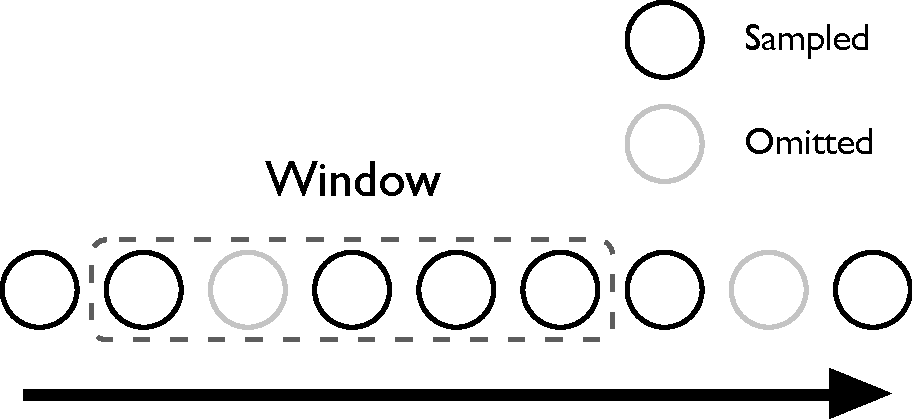
\includegraphics[scale=0.5]{pdf/stream.pdf}
	\caption{Stream querying.}
	\label{fig:stream}
\end{figure}

\subsection{Querying a Data Stream}

The assumption behind using a time window is that users of a real-time system are most likely interested in the most recent events. Sampling, on the other hand, is used to reduce the number of events used to answer a query \citep{Gaber:2005:MDS:1083784.1083789}. This way the system can keep up with the data and stay real-time.

Even though an answer to a query might be only approximate it can have great value because the query is answered at the right time. Furthermore, even though the query may only run on a subset of the data it is still possible to detect trends or system failures. For example, Twitter is using Apache Storm to perform real-time analysis on millions of events per second with their analytics product Answers \citep{Solovey}.

In research, several techniques have been developed to enable real-time data stream mining. For example, the MOA environment presented in \cite{Bifet:2010:MMO:1756006.1859903} which enables running online machine learning algorithms using the WEKA machine learning workbench \citep{Holmes1994}. In \cite{rainatwitter} authors present a real-time Opinion Mining (sentiment analysis) system built with Apache Storm and the Twitter Streaming API.

\section{Multi-core}
\label{sec:multicore}

\textcite{akhter2006multi} define multi-core processor as a processor that has two or more independent execution cores. This means that every thread has a hardware execution environment entirely to itself which enables threads to run in a truly parallel manner.

Running an application on multi-core can in the best case produce a speedup equivalent to the number of cores. The best case is when an application is embarrassingly parallel i.e. there is no inter-thread communication. Even though data stream processing is not an embarrassingly parallel problem, running a producer-consumer application on multiple cores can produce significant speedup, as shown in \citep{Prat-Perez:2013:PPM:2450027.2450037}.

\subsection{Advantages Over Clusters}
\label{subsec:advantages}

There are several reasons why someone might prefer to deploy their data stream application to a single multi-core machine rather than a cluster:

\begin{description}
	\item[Communication Overhead] \hfill \\
	The latency of over-the-network communication is significantly higher than that of processor cores communicating within a single machine.
	\item[Lower Cost than a Data Centre] \hfill \\
	To run a distributed system on a cluster one would usually first need to own a data centre. This comes with a high capital cost and increased maintenance costs compared to owning a single server.
	\item[More Control than with a Cloud Provider] \hfill \\
	Alternatively, one could rent out nodes on cloud computing services such as Amazon AWS or Rackspace. While the cost of such services is acceptable the user does not have full control over their system. This might be essential for high-security applications.
\end{description}

\subsection{Disadvantages Over Clusters}
\label{subsec:disadvantages}

On the other hand, there are certain disadvantages in deploying a data stream application to a single multi-core machine rather than a cluster:

\begin{description}
	\item[Horizontal Scaling] \hfill \\
	Commodity hardware clusters offer better horizontal scaling than a single multicore server. If one needs to add nodes to the cluster it is as easy as purchasing more commodity hardware. On a multi-core machine it is not that simple. For example, a top of the line Intel\textsuperscript{\textregistered} Xeon\textsuperscript{\textregistered} E5-2699 processor has support for 36 threads. Beyond that one would need to add another socket which essentially doubles the price. Moreover, the server would need to support multiple processor sockets.
	\item[Higher Short-term Cost than with a Cloud Provider] \hfill \\
	In short-term the cost of purchasing a server may be significantly higher than renting out a cluster from a cloud computing service. Thus, it makes most sense to run an application on multi-core as a medium- to long-term investment.
	\item[More Maintenance than with a Cloud Provider] \hfill \\
	Owning a server requires more maintenance than simply renting it out from a cloud provider. A cloud provider usually does  all the necessary maintenance and can easily provision a new machine. Hence it is advantageous to use a multi-core server only if one can afford to maintain it as well.
\end{description}

\section{Apache Storm}
\label{sec:apache_storm}

Apache Storm is an open source distributed real-time computation system. Storm was originally created by Nathan Marz while working at BackType \cite{NathanAbout}. BackType was later acquired by Twitter and Storm became open source. Storm was incubated into the Apache Software Foundation with version 0.9.1 and became a top-level Apache project in September 2014.

Storm was developed to run on top of a cluster where nodes execute components of a computation in parallel. Running Storm on a cluster of commodity hardware gives it good horizontal scaling properties. Running separate components in parallel allows the system to fully utilise available hardware and execute in real time.

\subsection{Dependencies}

Storm has five major dependencies:

\begin{description}
	\item[Apache Zookeeper] \hfill \\
	Apache Zookeeper \citep{ApacheZookeeper} is an open source server that allows reliable distributed coordination. Storm uses Apache Zookeeper to maintain state which is then read and written to by nodes of a Storm cluster. More details on how Storm uses Zookeeper are provided in section \ref{subsec:zookeeper}.
	\item[Apache Thrift] \hfill \\
	Apache Thrift \citep{ApacheThrift} is a cross-language framework for network services. It allows you to write a definition file for services and data types required by your application and it then automatically generates source code which supports remote procedure calls and serialisation of the data types.
	\item[Kryo] \hfill \\
	Kryo \citep{EsotericKryo} is a serialisation library. It is used to serialise objects before they are sent between nodes of a Storm cluster.
	\item[Netty] \hfill \\
	Netty \citep{Netty} is an asynchronous event-driven network application framework. Storm utilises Netty to send intra-cluster messages. Thus when a node produces a result to be consumed by another node of the cluster it sends a message over the network using the TCP protocol implemented in Netty.
	\item[LMAX Disruptor] \hfill \\
	LMAX Disruptor \cite{LMAXDisruptor} is a high-performance data structure used to exchange data between concurrent threads. It uses an optionally lock-free implementation of a ring buffer which Storm components running on the same node of a cluster use to exchange messages.
\end{description}

\subsection{Usage of Apache Storm}

Storm works particularly well with sister Apache projects such as Apache Kafka \cite{ApacheKafka} and Apache HBase \cite{ApacheHBase}. Apache Kafka is a messaging broker that is often used as the missing link between producers and consumers of a cluster. For example, web API endpoints might send data to a Kafka queue and a Storm application can then read the data from the queue. Apache HBase is a big data-store that allows real-time random reads and writes. It is modelled after Google's Bigtable project \cite{Chang:2008:BDS:1365815.1365816} and can be used to store data in a distributed way.

Storm is reportedly used by 81 companies listed on their ``Powered~By" website \cite{PoweredBy} and possibly many others. Storm's popularity is one of the reasons why it was chosen for this project. We also believe that the concepts used in Storm (explained in Section \ref{sec:concepts}) apply to a large number of different situations and many applications can be easily adapted to work on Storm.

There has been significant research into optimising computations running on Apache Storm. For example, \cite{Chatzistergiou:2014:FHN:2661829.2661882} looked at how to reconfigure a Storm job by reallocating component tasks to minimise communication cost, \cite{DBLP:conf/fedcsis/ChandrasekaranSA14} proposed a domain specific language for defining Storm jobs, and finally \cite{dimsonhailstorm} looked at how to provide exactly-once semantics in a Haskell port of Storm.

\section{Similar Efforts}
\label{sec:similar_efforts}

Currently data stream processing is a province of distributed systems such as the ones mentioned in the previous section. Most programming languages support parallel execution and while there are many open-source libraries that ease the process of writing parallel programs on a single multi-core machine such as OpenMPI \cite{OpenMPI} and OpenMP \cite{OpenMP} , none of them are tailored to data stream processing. Furthermore, these libraries usually require the programmer to do some of the heavy lifting rather than abstract it away.

Apache Hadoop is another open-source distributed system. However, it is used in offline batch processing rather than in online real-time processing. There has been effort to port Hadoop to multi-core in \citep{Kumar:2013:HSD:2536274.2536314} (Hone) as well as in \citep{ranger2007evaluating} (Phoenix). This research suggests that borrowing ideas from distributed systems and applying them in the context of multi-core has potential. However, to our knowledge there has not been effort to port Storm or any other distributed real-time data stream processing system to multi-core.

\section{Summary}

Distributed real-time computation systems such as Apache Storm provide programmers with abstractions that make it easy to implement data stream processing applications on top of a cluster. However, in case of single multi-core machines there are not any obvious open-source software choices. While there exist several libraries that allow programmers to parallelise their computations, they are not tailored to data stream processing.

Additionally, running these systems on a single multi-core server might have potential benefits as opposed to executing them on a cluster of commodity hardware.

